\afterpage{\null\newpage}
\chapter{Adaptive Sampling Theory\label{ch:chapter3}}


In this chapter, we investigate the theory of Adaptive Sampling with the goal to better understand the possibilities and limits of adaptive sampling. The results stated here were originally published in paper  including the figures in this chapter. The material in this chapter was first published in: 

\cite{Adstrategies2018} \textbf{Hruska, E.}; Abella, J. R.; N\"uske, F.;
Kavraki, L. E.; Clementi, C.; Quantitative
comparison of adaptive sampling methods
for protein dynamics. J. Chem. Phys.
2018, 149 


\section{Sampling Problem}

X
typical tiem steps 2-5fs, with GPUS below 1 microsecond/day paralelliazation

Anton cite for small system up to 100microseconds/day

timescales  
for biomolecus protein folding and other global strc
other global structural rearrangements of the order of
$$10^{-1}$$ - $$10^1$$s.
As a matter of fact, dynamics Eq. (1.1) naturally spends the vast majority of the time in
stable regions of the configuration space, i.e., energy minima. Crossing a barrier to get into
an adjacent minimum is energetically not favored, and is an extremely rare event: waiting
enough time for the event to occur is the only solution to the issue.


timescales  
for biomolecus protein folding and other global strc
other global structural rearrangements of the order of
$$10^{-1}$$ - $$10^1$$s.

Slower (rare) processes are associated with crossing high free energy barriers
(in an appropriate coordinate space) which is likely to take many trials and time to be
crossed, thus representing the typical bottleneck to MD simulations.


Clearly, it is extremely likely that computational resources might not be enough to
record a sufficiently long trajectory which ensures that minima-trapping eects have not
compromised a thorough sampling of the system configurational space. Computing power
should then be redirected toward sampling rare events, in order to minimize the time the
dynamical exploration spends trapped in the minima: the resulting strategies are known as
enhanced sampling techniques [33–38].


\begin{figure}[H]
  \centering
  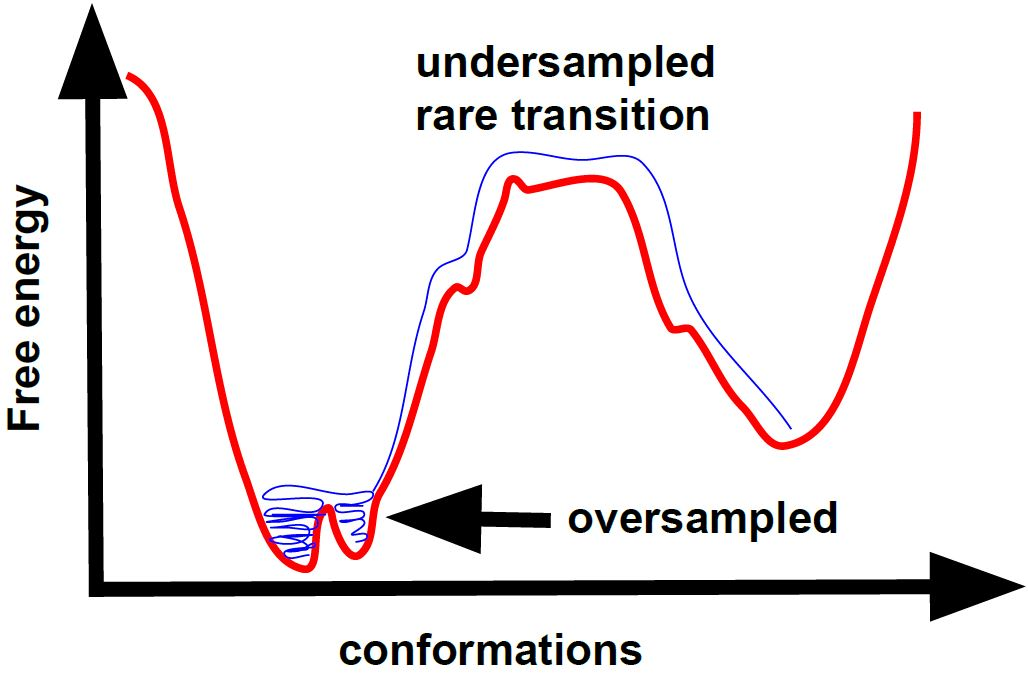
\includegraphics[width=0.9\linewidth]{figures3/rare_transition.pdf}
  \caption{rare transition}
  \label{fig:rare transitions}
\end{figure}


\section{\label{sec:intro2}Alternative sampling approaches}


The prevalent challenge of accurate sampling of the dynamics of high-dimensional stochastic systems  has led to many approaches, besides adaptive sampling.
These efforts can be broadly categorized, but this summary can not exhaustively discuss all approaches due to the large number of these approches.
One approach, is to simulate longer molecular dynamics trajectories by software and hardware approaches. In recent years the utilization of Graphics processing units (GPUs) and the design of special-purpose hardware \cite{shaw2014anton}. The graphics cards can currently simulate almost 1 microsecond of MD trajectory per day of simulation time for smaller proteins. The Special purpose hardware can simulate up to 100 microseconds of MD trajectory per simulation day, but the major limitation of the special-purpose hardware is the very limited access to these machines. A important role also played software advances which can effectively utilize these hardware. Despite all the improvements, these approaches perform simple molecular dynamics simulations and don't utilize the any additional possibilities of reaching longer timescales.

Another approach, incentivized by the increase in parallelization of High-Performance Computers is the simulation of many simultaneous trajectories \cite{DistComp-Shirts2000, DistComp-Buch2010}. The sampling is performed in parallel for the same system and by analyzing the resulting trajectories a better sampled result is obtained.  As shown in Chapter 4 the total efficiency of sampling is reduced due to the independend nature of the sampling, but the absolute simulation time or the time to solution is reduced.

Monte Carlo is a commonly used to improve the simulations of many stochastic systems. Here the sampling in not constrained to a hypersurface of conserved Hamiltonians, as is the case of molecular dynamics. This allows Monte Carlo to perform large jump in configuration space which is impossible in molecular dynamics. The high dimensionality of biomolecular systems reduces the effectivity of Monte Carlo Simulations which doesn't represent well the collective motions of biomolecules. The approach of Hybrid Monte Carlo attempts to combine the strength of both Monte Carlo and MD, by including information of the intermolecular forces in the Monte Carlo moves. This approach is promising, but wasn't yet able to increase the time-scales reachable. 


X
Altering the system's Hamiltonian is an approach common to multiple individual sampling methods. The common idea is modifying the Hamiltonian can lead to faster transitions and sampling and the stationary distribution for the original Hamiltonian can be extracted by subtracting the change in the Hamiltonian. In this class are approaches such as metadynamics \cite{laio2008metadynamics}, accelerated MD\cite{hamelberg2004accelerated}, replica-exchange MD \cite{sugita1999replica}. With these approaches the accurate kinetic information or conformational behavior cannot be directly extracted. Recently approaches such as Path reweighting methods \cite{pathreweight1, pathreweight2, pathreweight3, pathreweight4} have been introduced to help with the recovery of the dynamics, but haven't been widely used.


\section{\label{sec:intro2}Adaptive sampling approach}

The general idea of \emph{adaptive sampling} is the ``divide and conquer`` approach. Simulating shorter molecular dynamics trajectories allows to change the restarting points for the next short molecular dynamics trajectories. The choice of this restarting points is a key element of this thesis. Multiple approaches or \emph{adaptive sampling strategies} have been proposed before \cite{singhal2005error, bowman2010enhanced,
weber2011characterization, Fabritiis-2014, preto2014fast, doerr2016htmd,
AdaptivePELE-Lecina2017, EvolutionCoupling-Shamsi2017, FAST-Bowman-2015, 
Strategies-erros-reduce, plattner2017complete} and in the effectivity of different \emph{adaptive sampling strategies} will be investigated. At the end of adaptive sampling all the molecular dynamics trajectories are analyzed together which lead to the deside improved sampling or increased timescales obtainable. 



\begin{figure}[h]
  \centering
  \includegraphics[width=0.9\linewidth]{figures3/branching_picture.pdf}
  \caption{branching adaptive sampling}
  \label{fig:branching}
\end{figure}






The choide \emph{adaptive sampling strategies}
At each iteration, all of the simulations that have been performed at that
point are pooled and analyzed. New simulations are then initialized by
using the information extracted from the analysis of the previous iterations.
The main idea of adaptive sampling is that, by periodically analyzing the
conformational space already explored, new simulations can be restarted 
in a way that may significantly enhance the probability of observing rare
events. The choice of the strategy chosen to restart the trajectories is crucial
to the success of the approach, and several different methods have been
proposed \cite{weber2011characterization, Fabritiis-2014,
AdaptivePELE-Lecina2017,preto2014fast, doerr2016htmd,roblitz2013fuzzy,
weexplore, WESTPA-Zwier2015}.weber2011characterization
Recently, enhanced sampling in combination with adaptive sampling methods has
also been proposed~\cite{pathreweight5}.




 distributing them in a way to 
escape from local free energy minima, and efficiently visit different regions of
the conformational space of the systems of interest.

The advantage compared to other non-adaptive sampling strategies is the combination of accurate dynamics results and improved timescales reachable.

One common step of adaptive sampling is the necessity to 

 In the last decade, different methods have been
put forward to extract essential information from high dimensional MD data to a
small number of reaction coordinates associated with the slow
collective processes in the system's dynamics \cite{rohrdanz2013discovering,
noe2017collective}. Such methods include Markov State Models (MSMs) \cite{prinz2011markov,
MSM-Pande-2018,bookmsm,masterequationsMSM,SCHUTTE1999146}, Diffusion Maps
\cite{Coifman7426, rohrdanz2011determination,Zheng2011, Boninsegna2015}, likelihood based approaches
\cite{peters2006obtaining}, cut-based free energy profiles
\cite{krivov2008diffusive}, or neural networks \cite{Mardt2018,wehmeyer2018time,
ribeiro2018reweighted}.  

In particular, MSMs provide a good complement for
adaptive sampling as they are designed to handle many short trajectories and
do not require an equilibrium sampling to recover global thermodynamics and
kinetic properties (such as metastable states, free energy barriers, and
transitions between states), as long as the trajectories are in local
equilibrium.  

As mentioned above, different adaptive sampling methods can be characterized by how the
information extracted from previously explored space is used to
initiate new trajectories at each iteration.
Although the power of adaptive sampling has been demonstrated by successful
applications \cite{Wieczorek2016,Plattner20171005,Kohlhoff201415}, there is no general consensus as to how to
choose a particular method over another for a specific system. If the goal is
to simulate a rare event such as protein folding, does a method based on eigenvalues
outperform one based on counts? Could the same adaptive sampling method be then
used for general exploration of conformational space? Additionally, previous
studies \cite{preto2014fast,weber2011characterization,bowman2010enhanced,Fabritiis-2014} report efficiency gains with
adaptive sampling between a factor 2 and a factor of 10. What characteristics of the system of
interest can we use to predict that a particular adaptive sampling method will
provide a better efficiency gain?  Here we present a systematic study on a
number of model systems to address these questions.
In particular, we consider the efficiency of different adaptive sampling strategies for
two different goals on a number of model systems: to speedup the simulation
time needed to observe a specific rare event, such as the folding of a protein,
or to speedup the exploration of large regions of the conformational space of
the same protein.


Many different implementations of adaptive sampling exist but they all 
have in common
that the previous MD simulations are analyzed and restart points for the next
batch of MD simulations are determined from the analysis of the sampled configurational space.
The different implementations mainly differ in the analysis step, and
they can be based on Markov State Models (MSMs) \cite{prinz2011markov,
MSM-Pande-2018,bookmsm,masterequationsMSM,SCHUTTE1999146}, Diffusion Maps
\cite{Coifman7426, rohrdanz2011determination,Zheng2011, Boninsegna2015},
likelihood-based approaches \cite{peters2006obtaining}, cut-based free energy
profiles \cite{krivov2008diffusive}, or neural networks
\cite{Mardt2018,wehmeyer2018time, ribeiro2018reweighted}. 


In each iteration of Markov State Models-based adaptive sampling, all previous
MD simulations are analyzed.
Figure~\ref{fig:schema} is a graphical representation of the process. In the
first iteration of the adaptive sampling, the MD simulations are generated from
the system starting state as shown in Step 1.

In Step 2 all previous trajectories are analyzed. The first step is dimension reduction. One dimension reduction approach is using Time-lagged
Independent Component Analysis (TICA) \cite{TICA1-perez2013, TICA2-schwantes2013} converts the raw trajectories in
low-dimensional trajectories. The Koopman method \cite{koopmanold,
koopman2,koopman3,koopman4, wu2017variational, Nueske2017} is used to reduce
the non-equilibrium effects emerging from collecting many short MD trajectories. The
resulting low-dimensional trajectories are scaled into a kinetic map
\cite{Noe2015,noe2016commute}, which provides a measure of the kinetic distance
between different configurations. Another dimension reduction approach implemented by default in ExTASY is a deep learning approach with state-free reversible VAMPnets (SRV) \cite{Mardt2018,chen2019jcp}. The SRVs can effectively achieve non-linear dimension reductions. The SRV originates from the same variational
approach to conformational dynamics as TICA. The trajectory and the time-lagged trajectories are transformed with a neural network into dimension reduced trajectories. The dimension reduced trajectories are then used to calculate the VAMP-2 score, which is used as the loss function for the backpropagation to optimize the parameters of the neural network. The non-linear dimension reduction achieved with SRV improves the separation of different states. On advantage of SRVs is that SRVs can reach the same accuracy for time scales with shorter lag times than TICA. For adaptive sampling, the shorter lag time for analysis allows increasing the frequency of restarting trajectories which potentially improves adaptive sampling. In this case, the length of MD trajectories in each iteration is reduced and the number of iterations is increased.

The dimension reduced trajectories are then clustered with k-means into approximately 200 microstates,
the detailed values for each protein are provided in the Supplementary Information. 
A  maximum-likelihood estimation with a detailed balance
constraint \cite{prinz2011markov} allows obtaining an MSM transition matrix 
between every pair of microstates. All the analysis was
performed using the PyEMMA Python package \cite{scherer2015pyemma}, which
allows fast adjustments in the analysis step. The exact parameters for the MSM
construction for each protein are listed in the
Supplementary Information. All these steps can be modified or replaced easily in the
ExTASY workflow. 

Molecular dynamics (MD) simulations with all-atom force-fields allow simulating
protein folding and protein kinetics with good accuracy. Reaching biologically
relevant processes, such as protein folding or drug binding, is limited mainly
by the required large computational resources and long simulation times. The
long simulation times can be reduced either by simulating parallel trajectories
with massively-distributed computing \cite{DistComp-Shirts2000,
DistComp-Buch2010} or with special-purpose hardware \cite{shaw2014anton}.
Further reduction of required computational resources or simulation times would
allow a more broad application of MD simulations.

One method of reducing both the computational resources and the simulation times is \emph{adaptive sampling} \cite{singhal2005error, bowman2010enhanced,
weber2011characterization, Fabritiis-2014, preto2014fast, doerr2016htmd,
AdaptivePELE-Lecina2017, EvolutionCoupling-Shamsi2017, FAST-Bowman-2015, 
Strategies-erros-reduce, plattner2017complete, Adstrategies2018}. 
Adaptive sampling is an iterative process, where MD simulations from previous
iterations are analyzed, and, based on the analysis, a new iteration of relatively
short MD trajectories is initiated. The starting conformations for the
MD trajectories are determined in such a way to efficiently
reach a goal such as crossing rare transitions barriers, folding a protein, or
recovering the dynamics of a macromolecule. The exact strategy where to restart
new MD simulations determines the success of the adaptive sampling approach,
and several different methods have been proposed and investigated\GRE{\cite{Fabritiis-2014,
AdaptivePELE-Lecina2017, preto2014fast, doerr2016htmd,
weexplore, prattWESTPAAdvancesSampling2018, Adstrategies2018, FUNN, FAST}. One approach is to select new restarting configurations based on the PCA projection of the already sampled configurations \cite{shkurti2019jctc,harada2015jctc,harada2017jctc}.} Adaptive sampling
requires to use multiple parallel simulations and is therefore suitable for
High-Performance Computers (HPC).


\RED{ this section ok}
\section{\label{sec:design}ExTASY schematics}

This complexity of utilizing different software frameworks can detract from applying adaptive sampling or researching novel adaptive sampling methods. One method to reduce this complexity is to build the software in a modular approach. For ExTASY the modularity starts from splitting the adaptive sampling into individual steps shown in Figure~\ref{fig:schema2}.

\begin{figure}[h]
  \centering
  \includegraphics[width=0.5\linewidth]{figures2/schema1.pdf}
  \caption{Basic schema of adaptive sampling implemented in ExTASY. The
  number of starting conformations, the MD engines, and analysis strategies or Step 3 stop condition are flexible and can be changed. Identical schema to Figure~\ref{fig:schema}.}
  \label{fig:schema2}
\end{figure}

The individual adaptive sampling steps are summarized as follows:
\begin{itemize}
\item Start: Initialization of the start configurations.  Commonly an unfolded structure of the selected proteins is chosen.
\item Step 1: Simulating an ensemble of MD trajectories. The configurations chosen either by Initialization or Step 4. 
\item Step 2: Analysis of the all previously generated MD trajectories. The analysis varies between adaptive sampling strategies.
\item Step 3: Stop condition. Automatic determination if the objective of adaptive sampling is achieved. When the objective is not achieved, proceed iteratively to Step 4. 
\item Step 4: Selection of restart configurations for the next set of MD trajectories based on the analysis results 
\end{itemize}

The beginning step of any adaptive sampling is the initialization. The start configuration from where the adaptive sampling is launching is chosen. For each replica, which depends on the parallelization of the computational resource, a configuration is generated. The start configuration can be all identical or disparate. For proteins commonly a unfolded state is chosen.
In step 1 the MD simulations for all replicas is performed in a parallelized mode. Here most of the computational resources are utilized and scalability of this step is crucial. Commonly  
Following the MD simulation is the analysis of the MD trajectories in step 2. In ExTASY the flexibility python scripts allow the simple implementation and modification of different analysis strategies, including deep learning approaches\cite{Mardt2018}. In the following Chapters 5 and 6 the adaptive sampling strategies $cmicro$ and $cmacro$ with Markov State Models \cite{prinz2011markov} are used as described in Chapter 3. 

The results of Step 2 allow to determine in Step 3 if the objectives of adaptive sampling are reached. Examples for the objectives are protein folding, achieving a certain accuracy in protein dynamics or exploration of a part of the energy landscape corresponding to a smaller-scale motion of the protein. If the objective is not reached, Step 4 creates the restartings configuration for the next MD trajectories corresponding to Step 1. The adaptive sampling strategies to determine the restarting points in Step 4 in Figure~\ref{fig:schema2} are easily exchangeable, such as the strategies discussed in Chapter 2 or the FAST method \cite{FAST}. Once the objective in Step 3 is reached, adaptive sampling finishes and all trajectories can be further analyzed. 







\section{\label{sec:restart-strategies}Restart Strategies for Adaptive Sampling}

For each protein model, we use the MSM analysis and adaptive sampling procedure detailed
above with different restart strategies. We use a number of popular
strategies that do not assume a priori knowledge of the system, such as the microstate counts, or strategies that assume some a
priori knowledge of the system, such as the number of native contacts. 



Here we describe all the restart strategies that we have used on all the
different protein models. Several of these strategies require to set the value
of some parameters, which are provided in the Supplementary material. 

\subsection{plain MD} 

Comparison
As a reference, we generate synthetic MD trajectories without any adaptive
choice of the restart points. No analysis is performed after each
iteration, and each trajectory is restarted from the same state where it
ended in the previous iteration. That is, the restart state chosen for
trajectory $n_i$ at iteration $t$ is simply the state of trajectory $n_i$ at
iteration $t-1$.


\subsection{Adaptive sampling strategy $cmicro$}
One simple restart strategy is starting new molecular dynamics trajectories in
the microstates which have the worse statistics, that is, that have been visited the least during prior iterations
\cite{weber2011characterization, Fabritiis-2014, AdaptivePELE-Lecina2017,
doerr2016htmd}. This statement can be quantified by using the counts in the count matrix of the MSM from Step 2,
that report on how many times all previous trajectories have visited each
microstate.  The probability that any given microstate is selected in Step 4 for
the batch of restart conformations is inversely proportional to its associated count. The $cmicro$ strategy is effective in quickly exploring new regions of the whole protein landscape and to better sample the protein dynamics \cite{Adstrategies2018}.


\subsection{\label{sec:macro}Adaptive sampling strategy $cmacro$} 
Another popular restart strategy for adaptive sampling is a macrostate-based
method indicated here as $cmacro$. The main advantage of this
method is the faster folding of proteins or crossing of transition barriers
\cite{Adstrategies2018}. This advantage is achieved by using eigenvectors of
the on-the-fly MSM from Step 2 to select more restart configurations in areas which are
kinetically disconnected or less explored. In this method, the microstates of
the on-the-fly MSM are clustered into macrostates, for
example with PCCA \cite{roblitz2013fuzzy}. Any microstate not connected in the
main MSM is treated as an additional macrostate. The number of macrostates can
be either fixed, as in this work or determined based on the number of
slow processes emerging from the analysis. The macrostate count is determined by
measuring how many times any previous trajectory has visited each macrostate.
The restart conformations for the next iteration of adaptive sampling are then
chosen from each macrostate inversely proportional to the macrostate count.
Individual conformations within a macrostate are selected inversely
proportional to the microstate count within the macrostate.


\subsection{Cmicro adaptive sampling strategy ($1/C$)}
One intuitive and popular restart strategy consists in choosing the restart
states based on how many times the previous trajectories have visited each state
in the conformational space
\cite{weber2011characterization, Fabritiis-2014, AdaptivePELE-Lecina2017}, in
order to favor less populated states.  In particular, a
given state $i$ is chosen as restart state with a probability inversely
proportional to the number of times it has been visited.


\subsection{Cmacro adaptive sampling stategy ($1/C_M$)} 
Another count-based method that has been used in different applications clusters all the
visited microstates into fewer metastable macrostates on-the-fly. Usually, eigenvectors of
a matrix summarizing the sampling performed are used for the clustering
\cite{preto2014fast, doerr2016htmd}.  Here we use the transitions between all
the visited microstates to build an on-the-fly MSM, and the microstates are
clustered into macrostates using PCCA+ \cite{roblitz2013fuzzy}. 
%Any not fully connected microstates are treated as additional macrostates.
The restart state is then chosen with the following procedure. A macrostate
is first chosen with probability inversely proportional to the number of times
the macrostate has been visited. Then a microstate within the chosen macrostate
is chosen with probability inversely proportional to the number of times the
microstate has been visited. We have tested four variations of this strategy.
The first two variations (named $1/C_{M,1}^C$ and $1/C_{M,2}^C$) make use of the count
matrix $C_{ij}$ to directly estimate the on-the-fly MSM transition matrix. The count matrix
$C_{ij}$ contains the number of transitions that have been recorded in previous
iterations from state $i$ to state $j$. Every time a state is visited, the corresponding value
in the count matrix is incremented by one. This count matrix is normalized such
that each row sums to one and then used to estimate the on-the-fly MSM for the
adaptive sampling strategies.
The two variations differ as follows:
\begin{description}
\item[$1/C_{M,1}^C$]
PCCA+ is used to cluster the microstates into 30 macrostates.
\item[$1/C_{M,2}^C$]
The number of macrostates generated by PCCA+ is based on the number of
significant timescales using a 50\% kinetic content cutoff \cite{noe2016commute}.
\end{description}

The next two variations (named $1/C_{M,1}^K$ and $1/C_{M,2}^K$) are used to
estimate the effect of using non-equilibrium trajectories for the adaptive sampling
strategies. Since in most adaptive sampling methods many relatively short
trajectories are used, the non-equilibrium sampling can introduce errors in the
analysis of these trajectories.
Recently, the Koopman reweighting method
\cite{koopmanold, koopman2,koopman3,koopman4, wu2017variational, Nueske2017} has been
introduced to correct for the non-equilibrium effects in estimating global
equilibrium properties and can significantly reduce this error. In order to
evaluate the effect of the non-equilibrium sampling error in the performance of
the adaptive sampling strategy, we assume that the use of Koopman reweighting
in the analysis of MD trajectories can provide an accurate estimate of the
equilibrium transition probabilities between any pair of explored microstates.
Thus, in the synthetic trajectories used here, at each iteration, we estimate
an on-the-fly Koopman-corrected MSM by using the true transition probability
between the explored microstates (properly renormalized) and discarding any
transition to unexplored states.  Two more variants are studied by applying this correction to the previous two: 
\begin{description}
\item[$1/C_{M,1}^K$]
PCCA+ is used to cluster the microstates into 30 macrostates, on the Koopman-corrected MSM
\item[$1/C_{M,2}^K$]
The number of macrostates generated by PCCA+ on the Koopman-corrected MSM is
based on the number of significant timescales using a 50\% kinetic content
cutoff \cite{noe2016commute}.
\end{description}

adaptive sampling

\subsection{Adaptive sampling with a priori information}
If additional information is available on the system of interest, it can also be used to
guide the sampling. For instance, it has been proposed
\cite{EvolutionCoupling-Shamsi2017} to select restarting structures for
adaptive sampling based on the number of contacts likely made in the folded
states based on an evolutionary coupling analysis. Alternatively, the FAST
method \cite{FAST-Bowman-2015} was proposed as a way to exploit a priori
information, such as the distance to a target structure. 

\subsubsection{$Q_{f}$ - Native Contacts}
 Here, we
consider the case where the folded structure is known, and the number of native
contacts can be used as a reaction coordinate for the folding
process. Out of the states already visited by the simulation, states with a
higher median number of native contacts are chosen with higher probability than
states with a lower number of native contacts. The probability of choosing a
visited state $i$ is proportional to $exp( - k * | Q_i - Q_{max} | )$, where
$Q_i$ is the number of native contacts in state $i$, $Q_{max}$ is the total number of
native contacts, and $k$ is a parameter of the strategy (see Supplementary material).


\subsubsection{$Q_{f,nn}$ - Native and Non-native contacts} 
A variation of the previous strategy is to use two reaction coordinates in the
case when the folded structure is known, keeping track of the number of both
native and non-native contacts that are formed during the simulation. For each
state in the MSM, we compute the median number
of native and non-native contacts over all conformations mapped to each state.
Out of the states already visited by the simulation, states with a higher
number of native contacts have a higher probability of being chosen as
restarting points, as in the $Q_{f}$ strategy described above. Additionally,
states with a lower number of non-native contacts are chosen with a higher
probability than states with a higher number of non-native contacts. The
probability of choosing a visited state $i$ is proportional to $exp(-d_i)$,
where $d_i = \sqrt{k_1^2 * (Q_i - Q_{max})^2  + k_2^2 * N_i^2}$. $Q_i$
is the number of native contacts in state $i$, $Q_{max}$ is the total number of
native contacts, $N_i$ is the number of
non-native contacts in state $i$, and $k_1, k_2$ are parameters of the
strategy. One can think of $d_i$ as a distance to the folded state in
native/non-native contact space (scaled by $k_1$ and $k_2$). The two parameters
$k_1$ and $k_2$ were optimized by a parameter sweep (see Supplementary material). 
In real simulations such an optimization of the parameters is not
possible, but we perform it here to estimate the upper bound for the speed up.


\section{Upper limits to adaptive sampling strategies}

\subsection{$p_{esc}$ - Optimal strategy for exploration}
We also test a strategy that is not feasible in practice but offers a baseline
comparison as a theoretically optimal one. This strategy is built by using knowledge
of the full transition matrix of the system, that is not a priori known in real
applications (it is usually the goal of the sampling).
For each visited microstate $i$, we
compute the probability to transition to any microstate not yet explored using
the true transition matrix:
%
$$p_{esc}[i]=\sum_{j \in unexplored}T[i, j]$$
%
The state with the highest $p_{esc}$ value is chosen as the restart state. As stated above,
this strategy is impossible to implement in practice for real protein
simulations, but it is as a useful benchmark for comparing adaptive sampling
strategies that aim to explore conformational space.

\subsection{$t_{opt}$ - Optimal strategy to speedup slow processes (protein folding)} 
We also test another theoretically optimal strategy given perfect knowledge of the
system dynamics as well as knowledge of the folded states. In a way that is
similar to the definition of mean first passage time \cite{mfptbook},
for each state $i$ in the MSM, we compute a value $t_{opt}[i]$ which 
estimates the minimal time to reach the folded state.
We first define that for each folded state $f$, $t_{opt}[f] = 0$. Then we
iteratively solve the following recurrence relation for each state $i$ outside the folded region:
%
$$t_{opt}[i]=1+\sum_{j \in states}T[i,j]min(t_{opt}[i],t_{opt}[j])$$
%
The equation is solved iteratively until the relative change in $t_{opt}$ drops
below a cutoff. We then use it to define a benchmark restart strategy, by
selecting the restart state among the ones explored that has the lowest
$t_{opt}$ value, representing the state that is the closest to the folded
state. Note again that this strategy is impossible to implement in
practice, but still is a useful benchmark for adaptive sampling strategies.
With the $t_{opt}$ benchmark the maximum achievable speedup with adaptive
sampling for the folding of a protein can be evaluated.


\section{\label{sec:methods}Discussion}
preformance comparison ptomal to  othe strategies in next cahper




















